\documentclass[a4j,twocolumn]{jsarticle}
\usepackage{amssymb} % 高度な数式を表記するために使用
\usepackage[dvipdfmx]{graphicx}		% 図を入れるときに使用
\usepackage{wrapfig}		% 図の周りに本文を流し込みたいときに使用
\usepackage{url}
\usepackage{here}
\usepackage{subfigure}

\def\Vec#1{\mbox{\boldmath $#1$}}
\usepackage[dvipdfmx]{graphics}

\setlength{\textheight}{275mm}
\headheight 5mm
\topmargin -30mm
\textwidth 185mm
\oddsidemargin -15mm
\evensidemargin -15mm
\pagestyle{empty}

\begin{document}
\vskip 1.5em%

\title{三面図を利用した粒界原子配列の表示}
\author{関西学院大学 情報科学科 西谷研究室 1549 成田大樹}
\date{}
\maketitle

\section{序論}
原子間ポテンシャルを用いたシミュレーションの結果と大槻による実験結果の矛盾がある.具体的な相違点は,小傾角粒界エネルギーの0度,及び90度における立ち上がりの傾き方にある.原子間ポテンシャルを用いたシミュレーションの結果では,傾きが異なっているのに対し,大槻の実験結果では,傾きが左右対称である\cite{Otsuki}.

この矛盾を解明するために,西谷研究室では様々な手法をこれまで試してきた.最近の研究では,第一原理計算ソフトVASPを用いて構造緩和した結果,小傾角粒界エネルギーが大槻の結果を再現する程度の低いエネルギーを得た.しかし,外部格子全体に歪みが生じていたため,粒界傾角がより低い状態を計算していた\cite{Iwasa}.
この失敗は,安定構造の原子配列を視覚的に確認をしなかったことに起因する.
そこで,原子配列の視覚化を容易におこなうソフト開発を本研究では取り組んだ.

\section{ソフト開発の手法}
原子配列の出力は,原子座標を格納したPOSCAR形式のファイルを読み込んで,SVG形式で表示する.また.原子配列を三方向から投影した三面図で描画する.
これまで原子配列の構造は,図\ref{fig:one}のように,結晶構造描画ソフト”VESTA”を用いて3次元表示で確認してきた\cite{VESTA}.このソフトは原子構築を支援する汎用ソフトで,その表示は投影法により対象物を回転させて確認できるようになっている.しかし,今対象としている粒界においては,原子数が多いため個々の原子位置を判別しづらい.視点を固定した三面図での表示により,各面から原子の配置を直観的かつ確実に確認できるようになる.ただし,三面図の構成には規定があり,図面の各配置を遵守して描画しなければならない.

\begin{figure}[h]
\begin{center}
   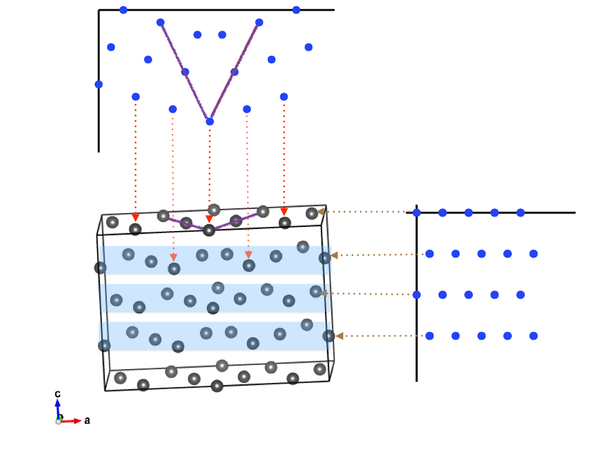
\includegraphics[width=55mm]{vesta_two_dimension.jpeg} 
     \caption{VESTAの投影図を2次元化した図.}
  \label{fig:one}
\end{center}
\end{figure}

\section{原子配列の表示結果}
ソフト開発をおこなう中で,様々な用途に合わせて原子配列を表示することが可能になった.まず,削除操作をおこなった原子配列の表示では,図\ref{fig:two}(a)のように,削除の有無によって原子の色と大きさを変えて描画した.その結果,削除された原子の個数ならびに各位置を視覚的に把握することができた.また,図\ref{fig:two}(b)のように,構造緩和による原子の移動を三面図で表示した.これにより,原子が移動した経路ならびに構造緩和に過ちが生じていないかを容易に確認することができるようになった. さらに,上面から見た各層の原子の位置を正確に把握するために,指定したz軸の層の原子を白抜きする機能を追加した.

\begin{figure}[H]
\subfigure[削除した原子の識別表示]
{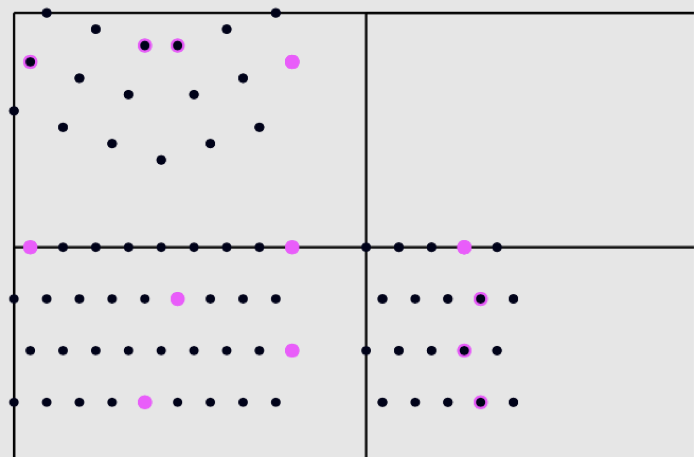
\includegraphics[keepaspectratio, width=44mm]
{./abst_fig2_a.png}}
\subfigure[構造緩和による原子移動]
{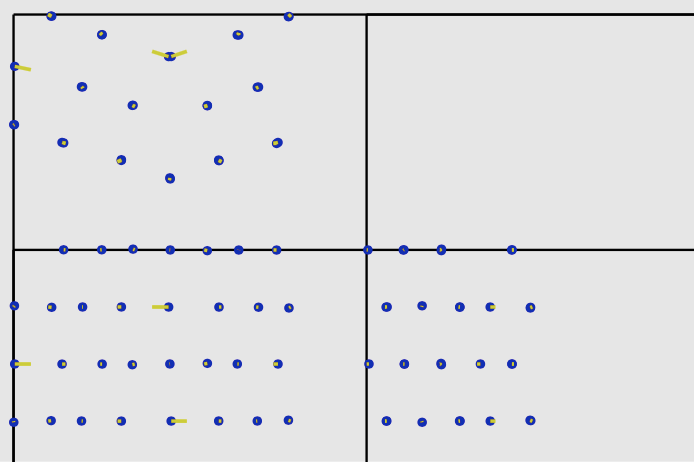
\includegraphics[keepaspectratio, width=44mm]
{./abst_fig2_b.png}}
\caption{{\footnotesize 三面図の表示例.}}
\label{fig:two}
\end{figure}

\section{まとめ}
三面図を用いて原子配列を表示したことにより,削除操作,および構造緩和をおこなった際の原子配置を視覚化することができた.また,構造緩和をおこなう際に使用したPOSCARファイルに過ちがあったことに気づいた.これは,今までのルーチンであった,原子配列の結晶構造描画ソフト"VESTA"による3次元表示では原子の細かい位置が確認できず,原子が不足していることを認識できなかったためである.このソフトの活用により,粒界原子配列の構造モデル構築が加速することが期待できる.

\begin{thebibliography}{9}
\bibitem{Otsuki} A. Otsuki, J. Material Science, 40(2005), 3219.
\bibitem{Iwasa} 岩佐恭佑 (関西学院大学 理工学部 学士論文 2016).
\bibitem{VESTA} VESTA, Koichi Momma, JP-Minerals, \url{http://jp-minerals.org/vesta/jp}, 2017/2/7アクセス.
\end{thebibliography}

\end{document}
